\subsection{Hierarchical clustering}\label{sec:hc}
The first algorithm considered for comparison is hierarchical clustering. Hierarchical clustering is a general family of clustering algorithms; they build nested clusters by merging or splitting them successively. This hierarchy of clusters can be represented as a tree or dendrogram. The root of the tree is the unique cluster that gathers all the samples, the leaves being the clusters with only one sample. To perform hierarchical clustering and merge the samples successively the \texttt{AgglomerativeClustering} function from \textit{scikit-learn} was used. Note that this approach was applied just to the samples, nothing was done to classify genes. In this case, genes are only dimensions in which samples are represented.

The \texttt{AgglomerativeClustering} object performs a hierarchical clustering using a bottom-up approach: each observation starts in its cluster, and clusters are successively merged. A linkage criterium determines the metric used for the merging strategy. 

First of all, distances between all elements are estimated; in this work standard euclidean distance was used. Then elements are merged using the linkage criterium; in this work standard \textit{Ward linkage} was used. The Ward linkage minimizes the sum of squared differences between the distances. It is a variance-minimizing approach. Here the specific configuration used in this work:
\begin{lstlisting}[style=mypython]
from sklearn.cluster import AgglomerativeClustering
AgglomerativeClustering(
    affinity='euclidean',
    compute_full_tree='auto',
    linkage='ward',
    n_clusters=x,
    )
\end{lstlisting}
note that the number of clusters is a free variable \texttt{\textbf{x}}: hierarchical clustering is not able to determine the ideal number of clusters. This was set from the output of the hierarchical Stochastic Block Model.
In figure~\ref{fig:topic/hc} an example of hierarchical clustering. Note that close nodes (with the euclidean distance defining \textit{close}) are linked firstly.
\begin{figure}[htb!]
	\centering
	\begin{minipage}{0.35\textwidth}
		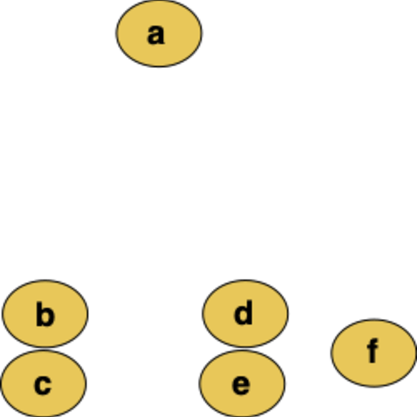
\includegraphics[width=0.8\linewidth]{pictures/topic/clusters.pdf}
	\end{minipage}
\hspace{3mm}
	\begin{minipage}{0.35\textwidth}
			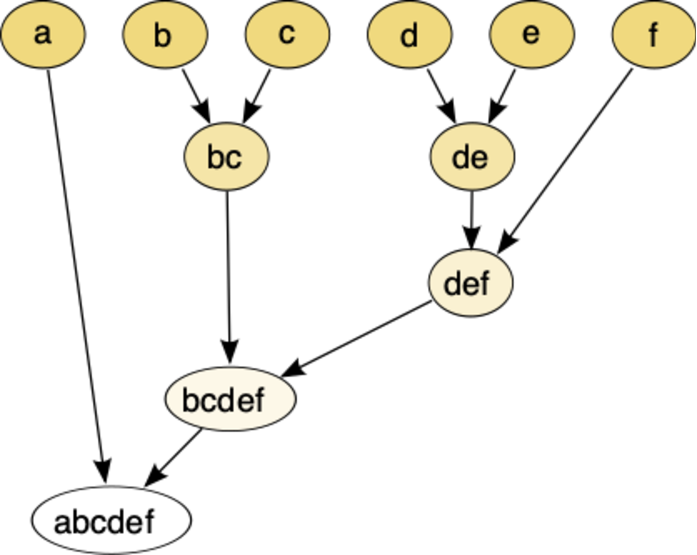
\includegraphics[width=0.9\linewidth]{pictures/topic/hierarchical_clustering_simple_diagram.pdf}
	\end{minipage}
\caption{Example of hierarchical clustering. Nodes are merged creating a tree (on the right).}
\label{fig:topic/hc}
\end{figure}

\subsection{Latent Dirichlet Allocation}\label{sec:lda}
Latent Dirichlet Allocation is the standard and well-known approach to topic models. It has got more restrictive priors than hierarchical Stochastic Block Model and needs some parameters to be set. It uses some different methods to maximize the posterior probability to observe some latent variables given the data.
As well described in~\cite{Zhou2016} LDA is a generative model and can be summarized as follows:
\begin{itemize}
	\item set the number of topics $K$ and the parameters $\eta$ and $\alpha$
	\item for each topic $k$ generate $\beta_k\sim \text{Dirichlet}(\bullet |\eta)$
	\item for each document $d$ generate $\theta_d\sim \text{Dirichlet}(\bullet|\alpha)$
	\item for each word in $d$ 
	\begin{itemize}
		\item generate $z\sim \text{Multinomial}(\bullet|\theta_d)$
		\item generate $w\sim \text{Multinomial}(\bullet|\beta_k)$
	\end{itemize}
\end{itemize}
\begin{figure}[htb!]
	\centering
	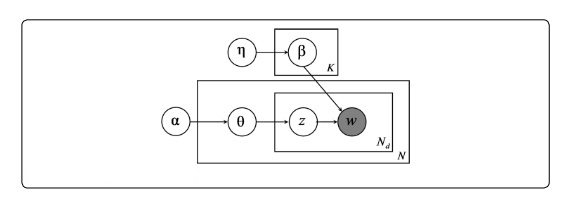
\includegraphics[width=0.65\linewidth]{pictures/topic/LDA.jpeg}
	\caption{LDA schematic representation.}
	\label{fig:LDA}
\end{figure}
this process is represented in figure~\ref{fig:LDA}. The goal is to maximize the posterior probability
\begin{equation}\label{eq:lda}
P(w, z,\beta, \theta| \alpha, \eta)=\prod_{d=1}^N P(\theta_d | \alpha)\prod_{n=1}^{N_d} P(w_{dn}|z_{dn},\beta_k)P(z_{dn}|\theta_d)\prod_{k=1}^KP(\beta_k|\eta)
\end{equation}
where
\begin{itemize}
	\item $N$ is the number of documents;
	\item $K$ is the number of topics as set by the user;
	\item $w$ are words;
	\item $N_d$ is the number of words in document d;
	\item $\alpha$ and $\eta$ are parameters of the model (usually $\eta=0.01$ and $\alpha=50/K$);
	\item $P(\theta | \alpha)$ and $P(\beta|\eta)$ are Dirichlet distributions.
\end{itemize}
When the distributions $\beta$, $\theta$ and $z$ are estimated, the outputs are the topic distribution in documents $P(\theta|\alpha)$ and the word distribution in topics $P(\beta|\eta)$.
Again the number of topics $K$ is not found by the model and needs to be set, this has been got from hierarchical Stochastic Block Model's output.